\documentclass{scrartcl}
\usepackage{graphicx}  % required for inserting images
\usepackage{float}

% for cyrillic and Bulgarian language
\usepackage[utf8]{inputenc}
\usepackage[T2A]{fontenc}
\usepackage[bulgarian]{babel}

% math packages
\usepackage{amsmath}
\usepackage{float}
\usepackage{amsfonts}
\usepackage{amssymb}

\usepackage{ragged2e}  % adds FlushLeft

\usepackage{mdframed}

\usepackage{listings}
\usepackage{xcolor}

\definecolor{codegreen}{rgb}{0,0.6,0}
\definecolor{codegray}{rgb}{0.5,0.5,0.5}
\definecolor{codepurple}{rgb}{0.58,0,0.82}
\definecolor{backcolour}{rgb}{0.95,0.95,0.92}

\lstdefinestyle{mystyle}{
    language=Octave,
    backgroundcolor=\color{backcolour},   
    commentstyle=\color{codegreen},
    keywordstyle=\color{magenta},
    numberstyle=\tiny\color{codegray},
    stringstyle=\color{codepurple},
    basicstyle=\ttfamily\footnotesize,
    breakatwhitespace=false,         
    breaklines=true,
    captionpos=b,
    keepspaces=false,                 
    %numbers=left,                    
    numbersep=5pt,
    showspaces=false,
    showstringspaces=false,
    showtabs=false,
    tabsize=2,
    basicstyle=\ttfamily\footnotesize,
    columns=fullflexible
}

\lstset{style=mystyle}

\title{Семинар 06}
\author{Ивайло Андреев}
\date{27 март 2025}

\begin{document}
\maketitle  % template title

\begin{flushleft}

\section{Увод към упражнението}

\subsection{Коплекситетът от непрекъснатостта}

Ще започнем днешното упражнението с отворен въпрос.

Кое е най-основополагащото нещо от ДИС-а?

\begin{mdframed}[linewidth=1.5pt, linecolor=black]
Кое е най-важното нещо от ДИС-а с една дума?
\end{mdframed}

Разбира се, вероятно верният отговор е нещо доста основно като например аритметични операции или понятието за функция. По-скоро въпросът се отнася за тези неща, които се учат от ДИС-а. Примерни отговори: интеграли, производни, порядъци, сходимост, ред, редица, криволинеен трапец и други.

\begin{mdframed}[linewidth=1.5pt, linecolor=black]
Отговорът, който аз ще дам, е \textbf{\textit{граница}}.
\end{mdframed}

Защо?
\begin{enumerate}
    \item Производна е по дефиниция граница.
    \item Неопределеният интеграл може да се разглежда като обратна операция на диференцирането (което казахме, че по дефиниция е просто граница), а определеният интеграл по дефиниция е граница на Риманови суми.
    \item Търсим сходимост чрез граници.
    \item Редици и редове са интересни заради граници.
\end{enumerate}

Границите обаче имат един проблем - не са тривиални.

\subsection{Сведения от числения анализ}

Нека разгледаме стандартната дефиниция за производна

$$f'(x) = \lim_{s\to 0}\dfrac{f(x+s)-f(x)}{s}$$

Имаме неопределеност от вида $\dfrac{0}{0}$ в общия случай и съответно диференцирането изисква доста повече отколкото просто елементарни математически операции.

Численият анализ ни казва, че можем да приближим точната стойност на производната (и в това число на всички нетривиални математически операции) с произволно малка грешка.

Нека $h$ е произволно малко

Тогава можем да приближим производната по следния начин

$$f'(x) = \lim_{s\to 0}\dfrac{f(x+s)-f(x)}{s} \approx \dfrac{f(x+h)-f(x)}{h}$$

За сега ще кажем само, че колкото по-малко е $h$, толкова по-близо сме до точната стойност и съответно толкова е по-малка грешката от приближението.

Имаме различни еквивалентни дефиниции за производна и когато използваме същата логика за приближение получаваме аналогично, но не еквивалентни приближения. Ето 3 подхода за числено диференциране:

\begin{enumerate}
    \item Разлика напред: $f'(x) = \displaystyle \lim_{s\to 0}\dfrac{f(x+s)-f(x)}{s} \approx \dfrac{f(x+h)-f(x)}{h}$
    \item Разлика назад: $f'(x) = \displaystyle \lim_{s\to 0}\dfrac{f(x)-f(x-s)}{s} \approx \dfrac{f(x)-f(x-h)}{h}$
    \item Централна разлика: $f'(x) = \displaystyle \lim_{s\to 0}\dfrac{f(x+s)-f(x-s)}{2s} \approx \dfrac{f(x+h)-f(x-h)}{2h}$
\end{enumerate}

Нека пак припомним, че всички тези числени приближение са точно това - \textbf{\textit{приближения}}. Доста съществен въпрос е каква е връзката между това колко малко $h$ използваме и каква грешка очакваме от приближението. По-конкретен въпрос е: "Ако намалим $h$ с дадена единица количество, то колко ще намалее грешката от приближението?". Така можем да говорим в порядъци.

Набързо само ще споменем грешката от вече споменатите числени диференцирания

\begin{enumerate}
    \item Разлика напред: грешка от порядъка на $O(h)$
    \item Разлика назад: грешка от порядъка на $O(h)$
    \item Централна разлика: грешка от порядъка на $O(h^2)$
\end{enumerate}

Повече подробности около грешки от числени методи се коментират в избираеми курсове за числени методи, включително "Теория на апроксимациите", "Числени методи за диференциални уравнения част първа", "Числени методи за диференциални уравнения част втора" и други.

\subsection{Възли и стойности}

Важно нещо, което трябва да отбележим е, че когато използваме числени методи за намиране на приближение на функция (например за намиране на интерполационен полином или намиране на решение на диференциално уравнение), то те НЕ ни дават (приближена) функция, на която да подадем произволни аргументи, а ни дават приближени стойности на решението в точни определени точки, който ще наричаме възли.

Затова въвеждаме означенията:
\begin{enumerate}
    \item Възли - точки по абсцисата (обикновено равноотдалечени), в които точки ще намираме приближение на решението.
    \item Стойности - приближената стойност на решението във възлите.
\end{enumerate}

Най-често възлите са равноотдалечени на разстояние от $h$ единици. Тоест когато намаляваме стъпката $h$ с цел да намалим грешката на приближенията, най-често ще се наложи да увеличим и броя възли и съответно броя стойности. Това ни подтиква да използваме софтуер за реализиране на числени методи. В рамките на този курс ще използваме MATLAB/Octave за тези цели.

\subsection{Octave за числата на Фибоначи}

Сега ще видим как можем да смятаме числата на Фибоначи с Octave. Ще направим това, защото числените методи за диференциални уравнения, които ще прилагаме после, са идейно много подобни.

Задачата е да намерим първите $N$ числа на Фибоначи, като напишем похдящ на Octave.

Няма да го направим рекурсивно, а итеративно. По-конкретно:

\begin{enumerate}
    \item инициализираме масив \textit{nodes} с първите 20 индекса, за който искаме да намерим числата на Фибоначи (т.е. от $0$ до $N-1$)
    \item инициализираме масив \textit{fibonacci-values} с празни елементи, всеки съответстващ на числото на Фибоначи за съответния индекс
    \item запълваме $F =$ \textit{fibonacci-values} по следната математическа схема:
    \begin{enumerate}
        \item $F_{0} = 0$
        \item $F_{1} = 1$
        \item $F_{i+1} = F_{i} + F_{i-1}\quad \forall i \ge 2$
    \end{enumerate}
\end{enumerate}

\lstinputlisting[language=Octave]{fib_code.m}

\begin{figure}[H]
    \centering
    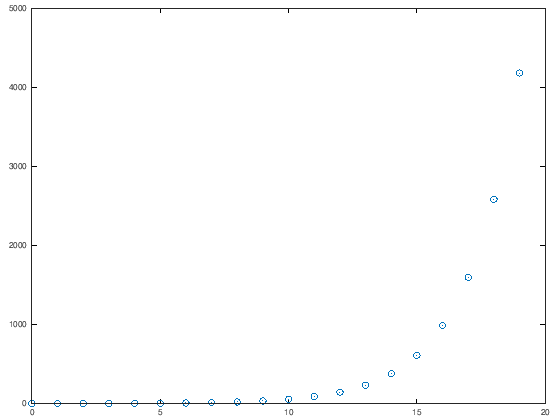
\includegraphics[width=0.8\textwidth]{fib_picture.png}
    \caption{Графика от кода}
    \label{fig:wolfram_sol}
\end{figure}

Общо взето това е нивото на код, нужно за имплементиране на числените методи за диференциални уравнения.

\end{flushleft}

\section{Метод на Ойлер}

\subsection{Общ случай}

Нека имаме следната задача на Коши

$$
\begin{cases}
y' = f(x, y)\\
y(x_0) = z_0
\end{cases}
$$

Ще я решим числено със следната схема.

Нека $x\in[x_0, A], \quad x_0<A\in\mathbb{R}$

Дефинираме следната мрежа: $x_i = x_0 + ih, \quad i = 0,\dots,N-1$, където $N\in\mathbb{N}$ и $h = \dfrac{A-x_0}{N}$

$N$ е броят възли и колкото по-голямо е $N$, толкова по-малко е $h$.

Предполагаме, че $y(x_i) \approx y_i$, тоест, че нашето приближение е приблизително равно на истинската стойност на решението в същата точка (с някаква грешка).

Численото решение, което решава задачата се задава със следната диференчна схема:

$$y_0 = z_0$$

$$y_{i+1} = y_{i} + h f(x_i, y_i)$$

\subsection{Извеждане на диференчната схема}

Ще я изведем с най-елементарните методи от числения анализ - числено приближение на производна. Хубаво е да отбележим, че има и подходяща геометрична интерпретация, която я има разписана в репото, но не и в този документ.

Имаме следното

\begin{align*}
\displaystyle f(x_i, y_i)
&= y'(x_i)\\
&\overset{def}{=} \displaystyle\lim_{s\to 0}\dfrac{y(x_i+s) - y(x_i)}{s}\\
&\approx \dfrac{y(x_i+h) - y(x_i)}{h}\\
&= \dfrac{y(x_{i+1}) - y(x_i)}{h}\\
&= \dfrac{y_{i+1} - y_i}{h}
\end{align*}

Така

$$y_{i+1} = y_i + h f(x_i, y_i)$$

\subsection{Конкретен пример}

Дадена е следната задача на Коши

$$
\begin{cases}
y' = x^2 - y^2\\
y(0) = 6
\end{cases}
$$

Да се намери приближение на решението с метода на Ойлер в интервала $x\in [0, 5]$ със стъпки $h = 0.1$, $h = 0.02$ и $h = 0.001$. Да се начертаят графиките на трите приближенията в една и съща координатна система.

\subsection{Решение на код}

\lstinputlisting[language=Octave]{euler.m}

\begin{figure}[H]
    \centering
    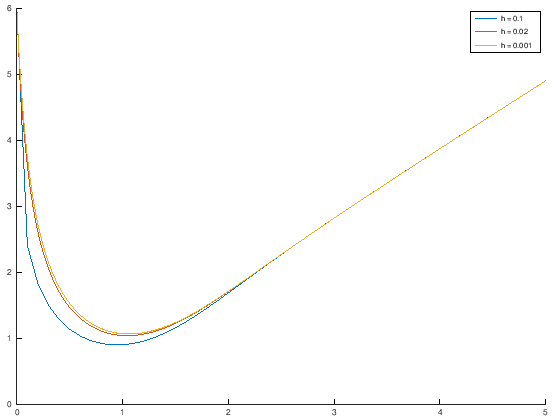
\includegraphics[width=0.8\textwidth]{euler_picture.png}
    \caption{Графики на приближените решения на задачата на Коши}
    \label{fig:euler_picture}
\end{figure}

\section{Числен метод за ОДУ от втори ред}

\subsection{Общ случай}

Нека имаме следната задача на Коши

$$
\begin{cases}
y'' = f(x, y, y')\\
y(x_0) = y_0\\
y(x_0) = z_0
\end{cases}
$$

Ще я решим числено със следната схема.

Нека $x\in[x_0, A], \quad x_0<A\in\mathbb{R}$

Дефинираме следнта мрежа: $x_i = x_0 + ih, \quad i = 0,\dots,N-1$, където $N\in\mathbb{N}$ и $h = \dfrac{A-x_0}{N}$

$N$ е броят възли и колкото по-голямо е $N$, толкова по-малко е $h$.

Предполагаме, че $y(x_i) \approx y_i$, тоест, че нашето приближение е приблизително равно на истинската стойност на решението в същата точка (с някаква грешка).

\subsection{Извеждане на диференчната схема}

Използваме следната формула за числено диференциране (разлика назад)

\begin{align*}
y'(x_i)
&= \lim \limits_{s\to 0} \dfrac{y(x_i) - y(x_i-s)}{s}\\
&\approx \dfrac{y(x_i) - y(x_i-h)}{h}\\
&= \dfrac{y(x_i) - y(x_{i-1})}{h}
\end{align*}

Така получаваме

$$y'(x_i) = \dfrac{y(x_i) - y(x_{i-1})}{h}$$

Диференцираме по $x_i$

$$y''(x_i) = \dfrac{y'(x_i) - y'(x_{i-1})}{h}$$

$y'(x_i)$ и $y'(x_{i-1})$ приближаваме с числено диференциране с разлика напред

\begin{align*}
y''(x_i)
&= \dfrac{\lim \limits_{s\to 0} \dfrac{y(x_i+s) - y(x_i)}{s} - \lim \limits_{s\to 0} \dfrac{y(x_{i-1}+s) - y(x_{i-1})}{s}}{h}\\
&\approx \dfrac{\dfrac{y(x_i+h) - y(x_i)}{h} - \dfrac{y(x_{i-1}+h) - y(x_{i-1})}{h}}{h}\\
&= \dfrac{y(x_i+h) - y(x_i) - y(x_{i-1}+h) + y(x_{i-1})}{h^2}\\
&= \dfrac{y(x_i+h) - y(x_{i}) - y(x_{i}) + y(x_{i-1})}{h^2}\\
&= \dfrac{y(x_{i+1}) - 2 y(x_{i}) + y(x_{i-1})}{h^2}\\
&\approx \dfrac{y_{i+1} - 2 y_{i} + y_{i-1}}{h^2}\\
\end{align*}

Така

$$y''(x_i) \approx \dfrac{y_{i+1} - 2 y_{i} + y_{i-1}}{h^2} = f(x_i, y_i, y'_i)$$

Откъдето

$$y_{i+1} = 2y_i - y_{i-1} + h^2f(x_i, y_i, y'_i)$$

$$y_{i+1} = 2y_i - y_{i-1} + h^2f\left(x_i, y_i, \dfrac{y_i - y_{i-1}}{h}\right)$$

Също имам начални условия

$$y_0 = y_0$$

$$\dfrac{y_1 - y_{0}}{h} = z_0$$

$$y_1 = hz_0 + y_0$$

Окончателно численото приближение, което решава задачата се задава със следната диференчна схема:

$$y_0 = y_0$$

$$y_1 = hz_0 + y_0$$

$$y_{i+1} = 2y_i - y_{i-1} + h^2f\left(x_i, y_i, \dfrac{y_i - y_{i-1}}{h}\right) \quad i=1,\dots,N-2$$

\subsection{Конкретен пример}

Дадена е задачата на Коши

$$
\begin{cases}
y''(x) = x^2 + xyy' + y'\\
y(0) = 1\\
y'(0) = 2
\end{cases}
$$

Да се намери приближение на решението с числен метод за ОДУ от втори ред в интервала $x\in [0, 5]$ със стъпки $h = 0.1$, $h = 0.02$ и $h = 0.001$. Да се начертаят графиките на трите приближенията в една и съща координатна система.

\subsection{Решение на код}

\lstinputlisting[language=Octave]{numeric_method.m}

\begin{figure}[H]
    \centering
    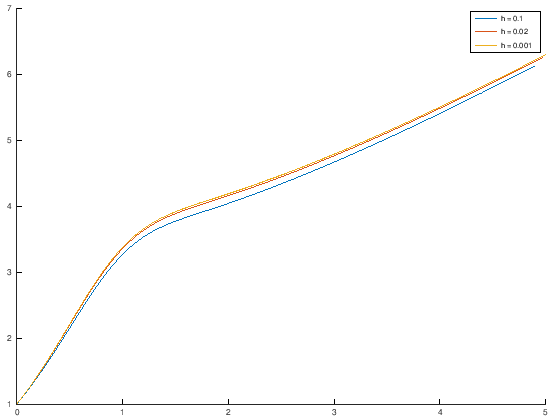
\includegraphics[width=0.8\textwidth]{numeric_method_picture.png}
    \caption{Графики на приближените решения на задачата на Коши}
    \label{fig:numeric_method_picture}
\end{figure}

\section{Метод на Пикар}

\subsection{Общ случай}

Имаме следната задача на Коши

$$
\begin{cases}
y'=f(y, x)\\
y(x_0) = y_0
\end{cases}
$$

Интегрираме уравнението формално, тоест в граници от $x_0$ до $x$.

$$\displaystyle \int \limits_{x_0}^{x} y'(t) \space dt = \int \limits_{x_0}^{x} f(y(t), t) \space dt$$

$$\displaystyle \int \limits_{x_0}^{x} \space dy(t) = \int \limits_{x_0}^{x} f(y(t), t) \space dt$$

$$\displaystyle y(x) - y(x_0) = \int \limits_{x_0}^{x} f(y(t), t) \space dt$$

$$\displaystyle y(x) = y(x_0) + \int \limits_{x_0}^{x} f(y(t), t) \space dt$$

$$\displaystyle y(x) = y_0 + \int \limits_{x_0}^{x} f(y(t), t) \space dt$$

Така сведохме задачата на Коши до *интегрално уравнение*. Това означава, че вече вместо да имаме уравнение с $y$ и $y'$, имаме уравнение само с $y$. Това ни позволява да направим последователни приближения, започвайки с $y_0$ от задачата на Коши и обща форма, която се задава по следния начин:

$$\displaystyle y_{i+1}(x) = y_0 + \int \limits_{x_0}^{x} f(y_{i}(t), t) \space dt$$

\subsection{Конкретен пример}

Дадена е следната задача на Коши

$$
\begin{cases}
y'=y\\
y(0) = 1
\end{cases}
$$

Да се намерят първите 5 приближения с метода на Пикар аналитично.

Да се начертаят с MATLAB/Octave в една координатна система графиките на първите 5 приближения на задачата на Коши по метода на Пикар в интервала $x\in[-2, 2]$.

\subsection{Аналично решение}

$$
\begin{cases}
y' = y, \\
y(0) = 1.
\end{cases}
$$

Интегралното уравнение по метода на Пикар е:

$$
\displaystyle y_{i+1}(x) = y_0 + \int \limits_{x_0}^{x} y_i(t) \space dt
$$

$$
\displaystyle y_{i+1}(x) = 1 + \int \limits_{0}^{x} y_i(t) \space dt
$$

\textit{Първо приближение}:

$$
y_0 = 1.
$$

\textit{Второ приближение}:

$$
y_1 = 1 + \int \limits_{0}^{x} 1 \space dt = 1 + \left[ t \right]_{0}^{x}.
$$

$$
y_1 = 1 + x.
$$

\textit{Трето приближение}:

$$
y_2 = 1 + \int \limits_{0}^{x} (1 + t) \space dt.
$$

$$
= 1 + \left[ t + \frac{t^2}{2} \right]_{0}^{x}.
$$

$$
y_2 = 1 + x + \frac{x^2}{2}.
$$

\textit{Четвърто приближение}:

$$
y_3 = 1 + \int \limits_{0}^{x} \left(1 + t + \frac{t^2}{2} \right) \space dt.
$$

$$
= 1 + \left[ t + \frac{t^2}{2} + \frac{t^3}{6} \right]_{0}^{x}.
$$

$$
y_3 = 1 + x + \frac{x^2}{2} + \frac{x^3}{6}.
$$

\textit{Пето приближение}:

$$
y_4 = 1 + \int \limits_{0}^{x} \left(1 + t + \frac{t^2}{2} + \frac{t^3}{6} \right) \space dt.
$$

$$
= 1 + \left[ t + \frac{t^2}{2} + \frac{t^3}{6} + \frac{t^4}{24} \right]_{0}^{x}.
$$

$$
y_4 = 1 + x + \frac{x^2}{2} + \frac{x^3}{6} + \frac{x^4}{24}.
$$

Така виждаме, че приближенията формират реда на Тейлър на $e^x$.

Също е добре да отбележим, че последователните приближения стават все по-точни в околност на точката $(x_0, y_0)$

\subsection{Решение на код}

\lstinputlisting[language=Octave]{pikar.m}

\begin{figure}[H]
    \centering
    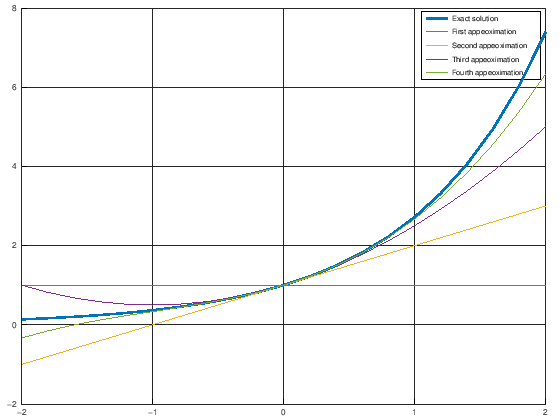
\includegraphics[width=0.8\textwidth]{pikar_picture.png}
    \caption{Графики на последователни приближени решения на задачата на Коши}
    \label{fig:pikar_picture}
\end{figure}

\section{Поле от прави}

\subsection{Общ случай}

Нека имаме диференциално уравнение от вида $y' = f(x, y)$

Ще построим поле от прави за него.

Избираме си мрежа от точки в равнината.

За всяка точка $(x_k, y_m)$ от мрежата ще разглеждаме следната задача на Коши

$$
\begin{cases}
y' = f(x, y)\\
y(x_k) = y_m
\end{cases}
$$

Няма да я решаваме обаче.

Ще построим отсечка с фиксирана дължина, която да минава през точката $(x_k, y_m)$. Нека тази дължина е $2\delta$.

\begin{figure}[H]
    \centering
    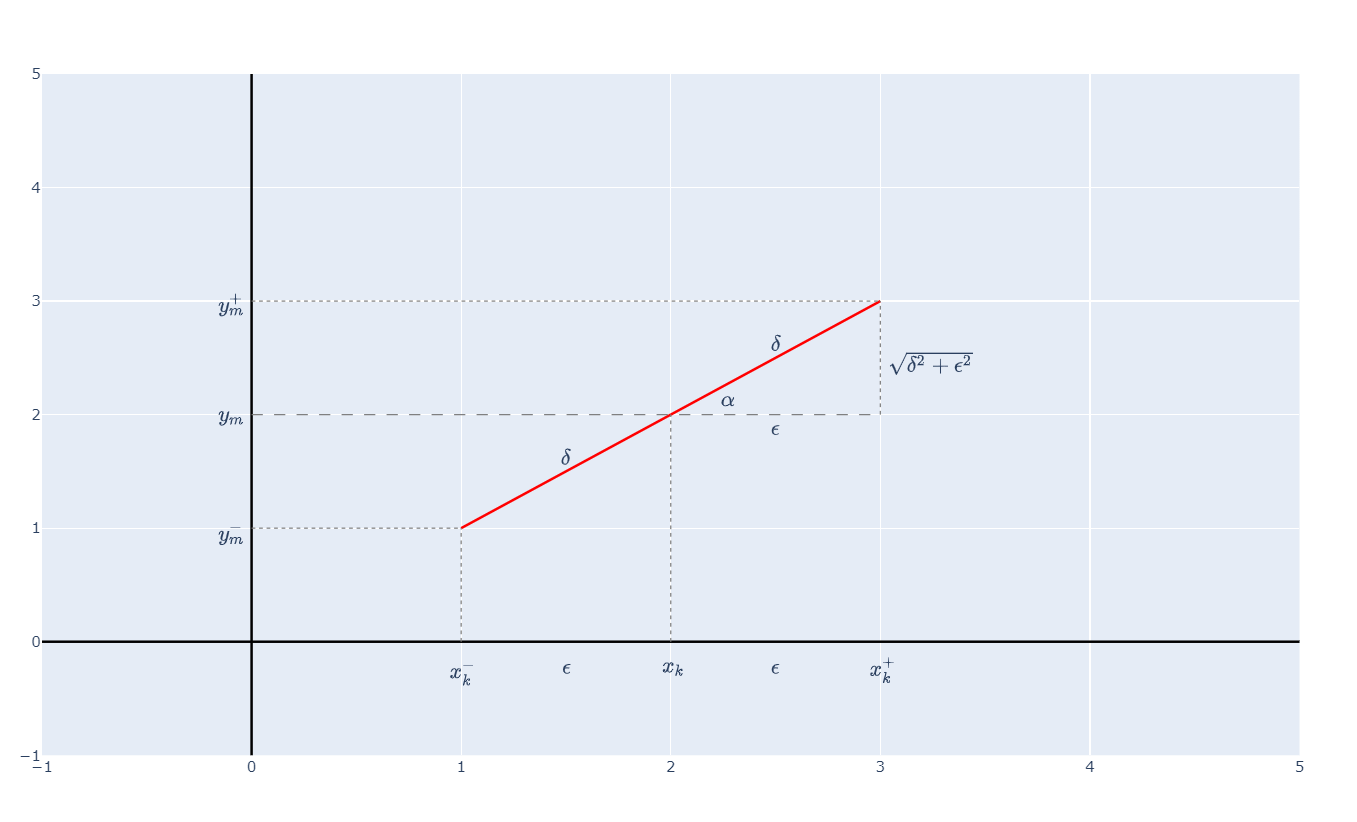
\includegraphics[width=0.8\textwidth]{slope_field_theory_picture.png}
    \caption{Графики на последователни приближени решения на задачата на Коши}
    \label{fig:slope_field_theory_picture}
\end{figure}

Знаем, че $y'(x_k) = \tan{\alpha}$

Така наклонът и дължината на отсечката са еднозначно определени.

Остава да открием точни координати за точките $(x_k^+, y_m^+)$ и $(x_k^-, y_m^-)$. Те са симетрични и е достатъчно да намерим координатите само на една от двете точки - например $(x_k^+, y_m^+)$

Означаваме с $\epsilon$ разстоянието между $x_k$ и $x_k^+$

С Питагорова теорема намираме третата страна на правоъгълния триъгълник горе дясно.

От тригонометричното определени за тангенс $\tan{\alpha} = \dfrac{\sqrt{\delta^2 + \epsilon^2}}{\epsilon}$

$$
\begin{cases}
y'(x_k) = f(x_k, y_m)\\
y'(x_k) = \tan{\alpha}\\
\tan{\alpha} = \dfrac{\sqrt{\delta^2 - \epsilon^2}}{\epsilon}
\end{cases}
$$

Значи

$$f(x_k, y_m) = \dfrac{\sqrt{\delta^2 - \epsilon^2}}{\epsilon}$$

$$f(x_k, y_m)^2 = \dfrac{\delta^2 - \epsilon^2}{\epsilon^2}$$

$$f(x_k, y_m)^2 + 1= \dfrac{\delta^2}{\epsilon^2}$$

$$\epsilon^2= \dfrac{\delta^2}{f(x_k, y_m)^2 + 1}$$

$$\epsilon= \dfrac{\delta}{\sqrt{f(x_k, y_m)^2 + 1}}$$

Намерихме $\epsilon$ и съответно можем да намерим $x$-координатата $x_k^+ = x_k + \epsilon$

Остава да намерим и $y$-координатата. Ще я намерим по следния начин

$$y_m^+ - y_m = \sqrt{\delta^2-\epsilon^2} = \epsilon f(x_k, y_m)$$

Откъдето

$$y_m^+ = y_m + \epsilon f(x_k, y_m)$$

\subsection{Конкретен пример}

Нека имаме следното диференциално уравнение:

$$y' = -\dfrac{y}{x}$$

\begin{enumerate}
    \item Да се начертае поле от прави за това ДУ в интервала $x\in[-5, 5], y\in[-5,5]$ с черен цвят.
    \item В същата координатна система начерайте графиката решението на задачата на Коши за даденото диференциално уравнение с начално условие $y(1.5) = -2$ с червен цвят.
\end{enumerate}

\subsection{Решение на код}

\lstinputlisting[language=Octave]{slope_field.m}

\begin{figure}[H]
    \centering
    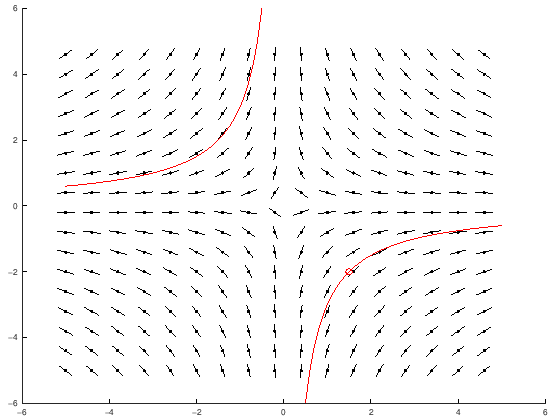
\includegraphics[width=0.8\textwidth]{slope_field_picture.png}
    \caption{Графики на поле от прави за даденото ДУ}
    \label{fig:slope_field_picture}
\end{figure}

\subsection{Допиралтелна към интегрална крива}

Нека имаме следната задача на Коши:

$$
\begin{cases}
y' = f(x, y)\\
y(x_0) = y_0
\end{cases}
$$

Производната $y'(x_0)$ в точката $x_0$ се изчислява като:  

$$y'(x_0) = f(x_0, y_0) = \tan{\alpha}$$

Това е наклонът $\tan{\alpha}$ на допирателната в точката $(x_0, y_0)$.

Права с наклон $\tan{\alpha}$, минаваща през $(x_0, y_0)$, се описва с:

$$y = x\tan{\alpha} + n$$

$$y = f(x_0, y_0)x + n$$

Тази права минава през точката $(x_0, y_0)$ и съответно имаме следното равенство:

$$y_0 = f(x_0, y_0)x_0 + n$$

Откъдето

$$n = y_0 - f(x_0, y_0)x_0$$

Заместваме в уравнението на правата:

$$y_0 = f(x_0, y_0)x_0 + y_0 - f(x_0, y_0)x_0$$

Уравнението на допирателната към интегралната крива окончателно е:

$$y = y_0 + f(x_0, y_0)(x - x_0)$$

\end{document}
